\fig{fv:k6:link}{相对速度垂直杆，相对加速度还含沿杆向内的分量}{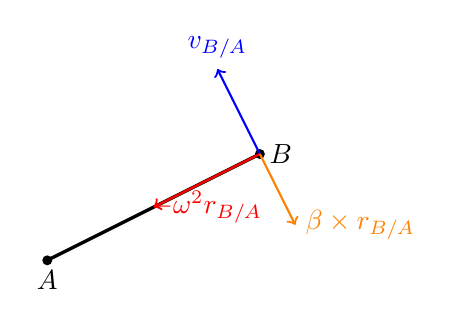
\begin{tikzpicture}[scale=.9]
\coordinate(A)at(0,0);\coordinate(B)at(3,1.5);\draw[very thick](A)--(B);\fill(A)circle(2pt)node[below]{$A$};\fill(B)circle(2pt)node[right]{$B$};
\draw[->,blue,thick](B)--(2.4,2.7)node[above]{$\bm v_{B/A}$};
\draw[->,red,thick](B)--(1.5,.75)node[midway,below]{$-\omega^2\bm r_{B/A}$};
\draw[->,orange,thick](B)--(3.5,.5)node[right]{$\bm\beta\times\bm r_{B/A}$};
\end{tikzpicture}}
图\ref{fv:k6:link}用同一根杆说明速度图不能直接充当加速度图。蓝箭头来自杆长不变，垂直 $AB$；橙箭头来自角速度大小变化；红箭头来自方向变化，始终沿 $BA$。只有将后两项与基点 $A$的加速度相加，才得到 $B$的对地加速度。即使驱动端匀速或某瞬间 $\beta=0$，红色项仍不能删去；机构接近死点时也应回到完整分量方程检查。
